\documentclass[11pt,a4paper,UTF8]{ctexart}
\ctexset{section = {format = \raggedright\Large\bfseries,}} %使\section中的内容左对齐 
%Premeable
	\usepackage[datesep=/]{datetime2}
\DeclareTextFontCommand{\textbf}{\sffamily}
%Presenting
\usepackage[table]{xcolor}
\usepackage{graphicx}
\usepackage[font={sf}]{caption}
\usepackage[above]{placeins}
\usepackage{float,wrapfig}
\usepackage{tabularx,array,booktabs,multirow,bigstrut}
\newcolumntype{C}[1]{>{\hsize=#1\hsize%
	\centering\arraybackslash}X}
\newcommand{\minitab}[2][l]{%
	\begin{tabular}{#1}#2\end{tabular}}
%MathSetting
\let\latexointop\ointop
\usepackage{amsmath,bm,amssymb,esint,extarrows}
\usepackage{upgreek,textcomp,mathrsfs}
\usepackage[only,sslash]{stmaryrd}
\usepackage{nicefrac,eqnarray}
%	\usepackage{amsthm}
\usepackage{mathtools,physics,siunitx}
\usepackage{stackengine,titling,varwidth}
\usepackage{tikz}
\usepackage{resizegather,empheq}
\usetagform{default}
\usepackage{calligra,fourier-orns}
% Keep \oint unchanged by esint
\let\ointop\undefined
\let\ointop\latexointop
% Define a scriptr 
\DeclareMathAlphabet{\mathcalligra}{T1}{calligra}{m}{n}
\DeclareFontShape{T1}{calligra}{m}{n}{<->s*[2.2]callig15}{}
\newcommand{\scriptr}{\mathcalligra{r}\,}
\newcommand{\rvector}{\pmb{\mathcalligra{r}}\,}
% Useful shorthand
\DeclarePairedDelimiter\ave{\langle}{\rangle}
\newcommand\inlineeqno{\stepcounter{equation}\ (\theequation)}
\newcommand{\sinc}{\operatorname{sinc}}
\newcommand{\mbb}[1]{\mathbb{#1}}
\newcommand{\mrm}[1]{\mathrm{#1}}
\newcommand{\mcal}[1]{\mathcal{#1}}
% Scaling and positioning
\newcommand\scalemath[2]{\scalebox{#1}{\mbox{\ensuremath{\displaystyle #2}}}}
\newcommand\raisemath[2]{\raisebox{#1\depth}{${#2}$}}
\empheqset{box=\bbox}
% Presenting
\newcommand*\bbox[1]{\fbox{\hspace{1em}\addstackgap[5pt]{#1}\hspace{1em}}}
\sisetup{%
	redefine-symbols=false,%
	separate-uncertainty=true,%
	range-phrase=\,\textasciitilde\,,%
	arc-separator = \,}
\allowdisplaybreaks[2]
%ParagraphSetting
\setlength{\parskip}{.3\baselineskip}
\usepackage[defaultlines=2,all]{nowidow}
\postdisplaypenalty=50
%PageSetting
\usepackage[colorlinks=true,linkcolor=blue]{hyperref}
\usepackage[vmargin={3cm,3cm},hmargin=2.8cm,%
	footnotesep=\baselineskip]{geometry}
\usepackage[bottom]{footmisc}
\usepackage{changepage}
% Autoref names
\renewcommand{\tableautorefname}{\tablename}
\renewcommand{\figureautorefname}{\figurename}
% List settings
\usepackage{enumitem}
\setlist{itemsep=0pt,topsep=0pt,labelindent=\parindent,leftmargin=0pt,itemindent=*}
% Some redefined lengths
\setlength{\headsep}{2.2cm}
\setlength{\droptitle}{-2.2cm}
\setlength{\footnotesep}{3\parskip}
% Header

% Separator
\newcommand{\newparagraph}{\pagebreak[3]\noindent%
	\hfil
	~\raisebox{-4pt}[10pt][10pt]{\decofourright~~~~~~~~\decofourleft}~ %
	\par
}
%TitleSettings
\pretitle{\begin{center}}
\posttitle{\par\end{center}\vspace{-6mm}}
\predate{}
\postdate{\vspace{-4mm}}
%Title
	\title{\textit{\large 基础物理实验}\\[2mm]
		\textbf{\LARGE 阻尼振动与受迫振动}}
	\author{\textit{未央书院能动} xx \textit{班 \ 江离 \ 学号} 202101xxxx}
	\date{}
%Miscellaneous
	\newcommand{\tabindent}{\hspace{2em}}
%FourierTransform
	\newcommand{\ftransform}{\xlongrightarrow{\ \mathscr F\ }}
	\newcommand{\iftransform}{\xlongrightarrow{\ \mathscr F^{-1}\ }}

\begin{document}
\tableofcontents
\maketitle

\section{摘要}

本实验利用波耳共振仪来探究阻尼振动、受迫振动与共振中的基本规律。观测不同阻尼对简谐振动的影响, 并使用最小二乘法线性拟合得出固有频率和不同阻尼下的阻尼系数;
分析受迫振动的基本规律, 测试幅度-频率特性和相位-频率特性,并得出共振频率和品质因数Q;探究振动系统在共振频率信号激励下从静止到稳态的过程,并作出振幅随时间变化的关系图。实验结果与理论预测相符。

\section{实验仪器}

带闪光灯的波耳共振仪一台。当进行周期测量,周期选择开关为 1 或 10 时, 周期不确定度分别为 $0.002 \mathrm{~s}$ 或 $0.0002 \mathrm{~s}$ 。

\section{实验内容}

\subsection{(A)观测有粘滞阻尼时的阻尼振动规律}

实验中使用波耳共振仪来探究粘滞阻尼下的振动规律。共振仪中的摆盘受到关于摆角$\theta$的线性回复力$F=-k\theta$以及正比于角速度的粘滞力$f=-\gamma\dot{\theta}$。设摆盘的转动惯量为$J$,可列出其运动方程:
	\[J\frac{\mathrm{d}^2 \theta}{\mathrm{d}t^2}=-k\theta-\gamma\dot{\theta}\tag{1}\]
若阻尼为零,则摆盘做简谐振动,固有频率$\omega_0=\sqrt{k/J}$。现设阻尼系数$\beta=\gamma/2J$(显然,这个物理量的量纲与$\omega_0$相同,即单位为$s^{-1}$),则这个方程可表示为:
	\[\frac{\mathrm{d}^{2} \theta}{\mathrm{d} t^{2}}+2 \beta \frac{\mathrm{d} \theta}{\mathrm{d} t}+\omega_{0}^{2} \theta=0\tag{2}\]
令方程的解为$\theta=\theta_0 e^{i\omega t+\varphi}$,代入原式可以解得
	\[\omega=\pm\sqrt{\omega_0^2-\beta^2}+i\beta\tag{3}\]
因此解有三种情况:
\\(1)欠阻尼($\beta<\omega_0$),这种情况的运动方程为
	\[\theta=\theta_{0} e^{-\beta t} \cos \left(\omega_{u} t+\varphi_{0}\right)\tag{4}\]
其中$\omega_u=\sqrt{\omega_0^2-\beta^2}$是欠阻尼下的振动频率,且此时振幅呈指数衰减。
\\(2)过阻尼($\beta>\omega_0$),这种情况的运动方程为
	\[\theta=e^{-\beta t}\left(\theta_{2} e^{\sqrt{\beta^{2}-\omega_{0}^{2}} t}+\theta_{3} e^{-\sqrt{\beta^{2}-\omega_{0}^{2}} t}\right)\tag{5}\]
(3)临界阻尼($\beta=\omega_0$),这种情况的运动方程为
	\[\theta=\theta_0e^{-\omega_0t}\tag{6}\]
此时摆盘回到平衡位置的时间最短。
\begin{figure}[h]
\centering
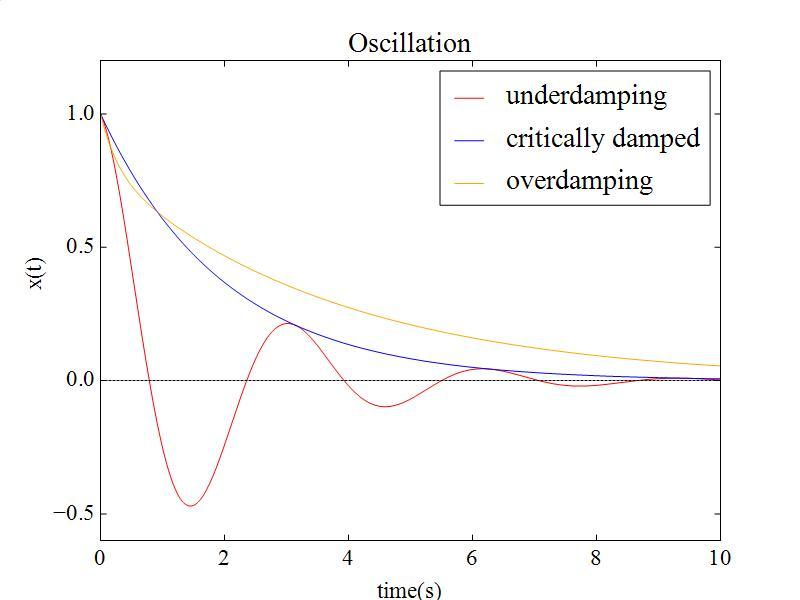
\includegraphics[width=.55\linewidth]{阻尼振动.jpg}
\caption{三种阻尼振动图示}
\end{figure}

现设法使摆盘处于欠阻尼状态,利用光电门测量每次振动的振幅和每十次摆盘经过平衡位置的时间间隔,便可粗略记录下振幅随时间的关系。实际上,假设每次振动的周期是
不变的,第$n$个周期后记录的振幅理论上应该是:
	\[\theta_n=\theta_0e^{-\beta(nT+t_0)}\tag{7}\]
其中$T$值理论上等于$\dfrac{2\pi}{\sqrt{\omega_0^2-\beta^2}}$。那么只要对上式取对数:
	\[\ln(\theta_n)=\ln(\theta_0)-\beta Tn-\beta t_0\tag{8}\]
便可通过最小二乘法将$\beta$计算出来。再结合求平均后得到的$T$值,就可以求出固有频率$\omega_0$。

实验对无外加阻尼、阻尼“2”档、阻尼“4”档三种情况振幅的振荡衰减过程进行记录。对无外加阻尼的情况,测量50次振幅(角度),并记录每十次振动用的时间,测量结果如下:
\begin{table}[H]
	\centering\caption{无外加阻尼条件下振幅与周期数据表}
	\small
	\begin{tabularx}{.85\textwidth}{ccccccccccc}
	\toprule
		振动次数 & \multicolumn{2}{c}{1-10} & \multicolumn{2}{c}{11-20} & \multicolumn{2}{c}{21-30} & \multicolumn{2}{c}{31-40} & \multicolumn{2}{c}{41-50} \\
	\midrule
		\multirow{5}*{振幅大小$\theta$/$^{\circ}$} & 150 & 145 & 139 & 135 & 131 & 127 & 121 & 118 & 114 & 110 \\
        	~ & 149 & 144 & 138 & 134 & 130 & 127 & 121 & 117 & 113 & 109 \\
		~ & 148 & 143 & 137 & 133 & 130 & 127 & 121 & 117 & 113 & 109 \\
		~ & 147 & 142 & 137 & 133 & 129 & 125 & 119 & 115 & 111 & 109 \\
		~ & 147 & 141 & 136 & 132 & 128 & 124 & 119 & 115 & 111 & 108 \\ \hline
		每十周期计时$T_{10}$/s & \multicolumn{2}{c}{15.365} & \multicolumn{2}{c}{15.380} & \multicolumn{2}{c}{15.394} & \multicolumn{2}{c}{15.402} & \multicolumn{2}{c}{15.413} \\
	\bottomrule
	\end{tabularx}
\end{table}
先求得十次周期平均值:$\overline{T_{10}}=\frac{15.365+15.380+15.394+15.402+15.413}{5}=15.391s$,忽略仪器系统误差
,标准偏差$s=\sqrt{\frac{\sum_{i=1}^{5}\left(T_{10i}-\overline{T_{10}}\right)^{2}}{(n-1)n}}=0.017s$
,$t$因子计算得$t_{0.95,4}=2.78$,从而A类不确定度$U_A=t_{0,95,4}\frac{s}{\sqrt{5}}=0.021s$,这远大于仪器误差限$\Delta_{INS}=0.002s$,因此不确定度可以只考虑A类分量。

故周期测量结果为$T=(1.5391\pm0.0021)s$。再对振幅的对数与振动次数进行线性拟合如下:
\begin{figure}[h]
	\centering
	\includegraphics[width=.8\linewidth]{线性1.png}
	\caption{无外加阻尼下$\ln(\theta)$与振动次数关系图}
\end{figure}

使用python的polyfit()函数可以得到$(8)$式中的斜率系数$\beta T=0.00680$,相关系数$r^2=0.9970$。
因此$\beta T$的A类不确定度$U_A=t_{0.95,48}\sqrt{\frac{RSS}{(n-2)\sum\left(\ln\theta_{i}-\overline{\ln\theta}\right)^{2}}}=0.00011$

则$\beta$的估值为$\frac{\beta T}{T}=\frac{0.00680}{1.5391}=4.42\times 10^{-3}s^{-1}$,不确定度为$U_{\beta}=\sqrt{(\frac{U_{\beta T}}{T})^2+(\frac{\beta TU_{T}}{T^2})^2}=7.2\times10^{-5}s^{-1}$,
即$\boxed{\beta=(4.42\pm0.07)\times10^{-3}s^{-1}}$,此即无外加阻尼(阻尼位于“0”档)时的阻尼系数。

同时,对固有频率我们还有公式:
	\[\omega_0=\sqrt{(\frac{2\pi}{T})^2+\beta^2}\tag{9}\]
在这里$\frac{2\pi}{T}=4.0823s^{-1}>>\beta$,因此可以忽略$\beta$的作用。固有频率的不确定度$U_{\omega_0}=\overline{\omega_0}\frac{U_T}{T}=0.0056s^{-1}$
,因此固有频率$\boxed{\omega_0=(4.082\pm0.006)s^{-1}}$。

现在对摆盘加上波耳共振仪自带的“2”档阻尼或“4”档阻尼。由于阻尼较大,此时振幅衰减的速率大大加快,因此每组只需记录8个振幅数据,以及4个周期数据。
下表为两种情况下记录的振幅和周期数据:
\begin{table}[H]
	\centering\caption{外加阻尼条件下振幅与周期数据表}
	\small
	\begin{tabularx}{.85\linewidth}{C{1} *8{C{.5}}}
	\toprule
		\textbf{阻尼“2”档} & 1 & 2 & 3 & 4 & 5 & 6 & 7 & 8 \\
	\midrule
		振幅$\theta$/$^{\circ}$     & 140  & 128  & 117 &  107  &  98  & 89 & 82 & 75  \\ \midrule
		周期/s    & \multicolumn{2}{c}{1.537} & \multicolumn{2}{c}{1.539} & \multicolumn{2}{c}{1.541} & \multicolumn{2}{c}{1.541}  \\
	\bottomrule
	\end{tabularx}
	
	\vspace{3ex}
	\begin{tabularx}{.85\linewidth}{C{1} *8{C{.5}}}
	\toprule
		\textbf{阻尼“4”档} & 1 & 2 & 3 & 4 & 5 & 6 & 7 & 8 \\
	\midrule
		振幅$\theta$/$^{\circ}$     & 111  & 94  & 79 &  66  &  55  & 47 & 39 & 33  \\ \midrule
		周期/s    & \multicolumn{2}{c}{1.541} & \multicolumn{2}{c}{1.543} & \multicolumn{2}{c}{1.545} & \multicolumn{2}{c}{1.545}  \\
	\bottomrule
	\end{tabularx}
\end{table}\noindent%

对两者振幅的对数与振动次数进行线性拟合如下:
\begin{figure}[h]
	\centering
	\begin{minipage}[t]{0.48\textwidth}
	\centering
	\includegraphics[width=7.2cm]{线性2.png}
	\caption{阻尼“2”档$\ln(\theta)$与振动次数关系图}
	\end{minipage}
	\begin{minipage}[t]{0.48\textwidth}
	\centering
	\includegraphics[width=7.2cm]{线性3.png}
	\caption{阻尼“4”档$\ln(\theta)$与振动次数关系图}
	\end{minipage}
\end{figure}

两种情况下的周期估值为$\overline{T_{2}}=\frac{1.537+1.539+1.541+1.541}{4}=1.5395s$,$\overline{T_4}=\frac{1.541+1.543+1.545+1.545}{4}=1.5435s$,
标准偏差$s_{T_2}=\sqrt{\frac{\sum_{i=1}^{4}\left(T_{2i}-\overline{T_{2}}\right)^{2}}{(n-1)n}}=0.00166s,s_{T_4}=\sqrt{\frac{\sum_{i=1}^{4}\left(T_{4i}-\overline{T_{4}}\right)^{2}}{(n-1)n}}$ $=0.00166s$
,$t$因子计算得$t_{0.95,3}=3.20$,从而A类不确定度$U_{T_2A}=U_{T_4A}=t_{0,95,3}\frac{s}{\sqrt{4}}=0.0027s$,即两种情况下的周期分别为$T_2=(1.5395\pm0.0027)s,T_4=(1.5435\pm0.0027)s$。

同时,使用python的polyfit()函数可以得到两种情况中$(8)$式中的斜率系数$\beta_2 T_2=0.0893,\beta_4 T_4=0.1742$,相关系数$r_2^2=0.99987,r_4^2=0.99982$。
因此两种情况下$\beta T$的A类不确定度$U_{2A}=t_{0.95,6}\sqrt{\frac{RSS}{(n-2)\sum\left(\ln\theta_{2i}-\overline{\ln\theta_2}\right)^{2}}}=0.0017$
,$U_{4A}=t_{0.95,6}\sqrt{\frac{RSS}{(n-2)\sum\left(\ln\theta_{4i}-\overline{\ln\theta_4}\right)^{2}}}=0.0041$。

则两种情况下$\beta$的估值分别为$\beta_2=\frac{\beta_2 T_2}{T_2}=\frac{0.0893}{1.5395}=0.0580 s^{-1}$,$\beta_4=\frac{\beta_4 T_4}{T_4}=\frac{0.1742}{1.5435}=0.1129 s^{-1}$
,不确定度为$U_{2}=\sqrt{(\frac{U_{\beta_2 T_2}}{T_2})^2+(\frac{\beta_2 T_2U_{T_2}}{T_2^2})^2}=0.0011s^{-1}$,$U_{4}=\sqrt{(\frac{U_{\beta_4 T_4}}{T_4})^2+(\frac{\beta_4 T_4U_{T_4}}{T_4^2})^2}$ $=0.0027s^{-1}$。
即$\boxed{\beta_2=(0.0580\pm0.0011)s^{-1}}$,$\boxed{\beta_4=(0.1129\pm0.0027)s^{-1}}$ 分别是阻尼挡位位于“2”和“4”时的阻尼系数。

接下来我们来讨论这些阻尼振动的品质因数。品质因数是衡量振动系统能量变化快慢的一个比值,数值上定义为$2\pi\dfrac{E}{|\Delta E|}$,其中$E$是振动系统存储的能量,
$\Delta E$是一个周期内振动能量的变化值。对于阻尼振动,一个周期内能量减小$k(x_n^2-x_{n-1}^2)$,其中$x$是振幅。那么在本实验的条件下有:
	\[Q=2\pi\frac{k\theta_n^2}{k\theta_n^2-k\theta_{n-1}^2}=\frac{2\pi}{1-(\frac{\theta_{n-1}}{\theta_n})^2}=\frac{2\pi}{1-e^{-2\beta T}}\tag{10}\]
如果阻尼较小,那么上式就可以简化成:
	\[Q\approx\frac{2\pi}{2\beta T}=\frac{\omega}{2\beta}\approx\frac{\omega_0}{2\beta}\tag{11}\]
即$Q$与阻尼系数$\beta$呈反比。根据这个公式,无外加阻尼、阻尼“2”档和阻尼“4”档下阻尼振动的品质因数估值分别为:
$\overline{Q_0}=\frac{\omega_0}{2\beta_0}=\frac{4.082}{2\times4.42\times10^{-3}}=462$,$\overline{Q_2}=\frac{\omega_2}{2\beta_2}=\frac{4.082}{2\times0.0580}=35.2$,$\overline{Q_4}=\frac{\omega_4}{2\beta_4}=\frac{4.082}{2\times0.1129}=18.08$。
它们的不确定度可以用$U_Q=Q\sqrt{(\frac{U_{\omega_0}}{\omega_0})^2+(\frac{U_{\beta}}{\beta})^2}$表示,因此
$U_{Q0}=462\sqrt{(\frac{0.006}{4.082})^2+(\frac{0.07}{4.42})^2}=7.3$,$U_{Q2}=35.2\sqrt{(\frac{0.006}{4.082})^2+(\frac{0.0011}{0.0580})^2}=0.67$,$U_{Q0}=18.08\sqrt{(\frac{0.006}{4.082})^2+(\frac{0.0027}{0.1129})^2}=0.43$。

因此无外加阻尼、阻尼“2”档和阻尼“4”档下阻尼振动的品质因数分别为:
$\boxed{Q_0=462\pm7}$,$\boxed{Q_2=35.2\pm0.7}$和$\boxed{Q_4=18.1\pm0.4}$。

\subsection{(B)分析振动系统受迫振动的基本规律, 观测幅频特性}

如果当振动系统在受到回复力$-k\theta$和粘滞阻尼$-\gamma\dot{\theta}$的同时,还受到一个周期性强迫力$F=A_f\cos(\omega_f t)$的作用,此时的振动系统运动方程可表示为:
	\[J\frac{\mathrm{d}^2 \theta}{\mathrm{d}t^2}=-k\theta-\gamma\dot{\theta}+A_f\cos(\omega_f t)\tag{12}\]
仍令$\beta=\gamma/2J$,$\omega_0=\sqrt{k/J}$。在欠阻尼条件下,上式的通解为:
	\[\theta=\theta_{0} e^{-\beta t} \cos \left(\sqrt{\omega_{0}^{2}-\beta^{2}} t+\varphi_{0}\right)+\theta_{e} \cos (\omega_f t-\varphi)\tag{13}\]
解包含了一个指数衰减的振荡项和一个简谐项。后者的频率与强迫力频率相同,其振幅为
	\[\theta_e=\frac{\omega_{0}^{2} A_{f}}{\sqrt{\left(\omega_{0}^{2}-\omega_f^{2}\right)^{2}+(2\beta \omega_f)^{2}}}\tag{14}\]
以及,这个简谐振动总是落后于强迫力一个相位差:
	\[\varphi=\arctan{\frac{2\beta\omega_f}{\omega_0^2-\omega_f^2}}\tag{15}\]
当受迫振动达到稳态后系统将只剩下这个振动。

由振幅的表达式知道,当强迫力频率$\omega_f$等于$\sqrt{\omega_0^2-2\beta^2}$时,稳态振幅达到最大,这称为共振现象。\textbf{若阻尼较小,$\beta<<\omega_0$,则共振频率近似等于固有频率}。
此时稳态下的振幅为$\theta_r=\frac{\omega_0^2A_f}{2\beta\sqrt{\omega^2_0-\beta^2}}\approx QA_f$,即近似为品质因数与强迫力振幅的乘积;
稳态下的相位差为$\varphi_r=\arctan{\frac{\omega_f}{\beta}}\approx\pi/2$,即近似落后$90^{\circ}$相位。

这能否得到实验的验证呢?通过画出受迫振动振幅和相位相对强迫力频率的幅频和相频曲线可以回答这个问题。

本部分实验通过波耳共振仪来实现不同频率的受迫振动,并测量相应的稳态振幅大小和相位差,画出共振点附近的幅频和相频曲线并与理论结果对照。本实验按阻尼大小分为“2”档和“4”档两组。
在实验中,\textbf{当仪器测量出的振幅不再变化,且闪光灯在盘面上照射出的刻度不再移动,即认为受迫振动已达到稳态},此时就可以记录下振幅大小和相位差数据。实验数据如下:

\begin{table}[H]
	\centering\caption{受迫振动中稳态振幅和相位与强迫力频率关系表}
	\small
	\begin{tabularx}{.95\textwidth}{c|ccc|c|ccc}
	\toprule
	\textbf{阻尼“2”档} & 周期/s & 振幅/$^{\circ}$ & 相位差/$^{\circ}$ & \textbf{阻尼“4”档} & 周期/s & 振幅/$^{\circ}$ & 相位差/$^{\circ}$ \\
	\midrule
	& 1.538 & 151 & 86 & & 1.434 & 25 & 159 \\ 
	& 1.545 & 145 & 71 & & 1.461 & 32 & 152 \\
	& 1.552 & 131 & 58 & & 1.485 & 43 & 147 \\
	& 1.559 & 119 & 49 & & 1.500 & 53 & 139 \\
	& 1.565 & 107 & 43 & & 1.515 & 64 & 128 \\
	& 1.578 & 84 & 35 & & 1.525 & 71 & 118 \\
	& 1.591 & 71 & 28 & & 1.533 & 77 & 107 \\
	& 1.608 & 55 & 23 & & 1.541 & 80 & 96 \\
	& 1.629 & 45 & 15 & & 1.549 & 81 & 85 \\
	& 1.652 & 36 & 12 & & 1.560 & 77 & 73 \\
	& 1.531 & 146 & 108 & & 1.571 & 71 & 61 \\
	& 1.524 & 123 & 119 & & 1.584 & 63 & 51 \\
	& 1.515 & 89 & 143 & & 1.605 & 51 & 40 \\
	& 1.501 & 65 & 156 & & 1.626 & 42 & 33 \\
	& 1.485 & 49 & 163 & & 1.651 & 34 & 29 \\
	& 1.459 & 34 & 168 & & & & \\
	& 1.433 & 26 & 171 & & & & \\
	\bottomrule
	\end{tabularx}
\end{table}

根据实验数据,阻尼为“2”档时强迫力频率在固有频率附近的幅频和相频特性曲线如下:
\begin{figure}[h]
	\centering
	\begin{minipage}[t]{0.48\textwidth}
	\centering
	\includegraphics[width=7.5cm]{幅频2.png}
	\caption{阻尼“2”档下受迫振动振幅与强迫力频率关系图}
	\end{minipage}
	\begin{minipage}[t]{0.48\textwidth}
	\centering
	\includegraphics[width=7.5cm]{相频2.png}
	\caption{阻尼“2”档下受迫振动与强迫力的相位差与频率关系图}
	\end{minipage}
\end{figure}

阻尼为“4”档时强迫力频率在固有频率附近的幅频和相频特性曲线如下:
根据实验数据,阻尼为“2”档时强迫力频率在固有频率附近的幅频和相频特性曲线如下:
\begin{figure}[h]
	\centering
	\begin{minipage}[t]{0.48\textwidth}
	\centering
	\includegraphics[width=7.5cm]{幅频4.png}
	\caption{阻尼“4”档下受迫振动振幅与强迫力频率关系图}
	\end{minipage}
	\begin{minipage}[t]{0.48\textwidth}
	\centering
	\includegraphics[width=7.5cm]{相频4.png}
	\caption{阻尼“4”档下受迫振动与强迫力的相位差与频率关系图}
	\end{minipage}
\end{figure}

下图是两种阻尼情况下的幅频和相频曲线,绿线为阻尼“2”档时的曲线,蓝线为阻尼“4”档时的曲线。从曲线图上可以读出,两种情况下振幅最大(共振)时强迫力频率
分别是$\omega_{r2}=4.085s^{-1},\omega_{r4}=4.061s^{-1}$,振幅为最大振幅的$\frac{\sqrt{2}}{2}$倍时强迫力频率分别是
$\omega_{2-}=4.015s^{-1},\omega_{2+}=4.135s^{-1},\omega_{4-}=3.982s^{-1},\omega_{4+}=4.172s^{-1}$。根据受迫振动品质因数的表达式
$Q=\frac{\omega_r}{|\omega_{+} -\omega_{-}|}$,代入上述数据可以得到阻尼“2”档和“4”档的品质因数分别是$\boxed{Q_2=34.0}$,$\boxed{Q_4=21.4}$,与A部分的结果相近。

\begin{figure}[H]
	\centering
	\includegraphics[width=.8\linewidth]{幅频24.png}
	\caption{不同阻尼系数下受迫振动振幅与强迫力频率关系图}
\end{figure}

\begin{figure}[H]
	\centering
	\includegraphics[width=.8\linewidth]{相频24.png}
	\caption{不同阻尼系数下受迫振动与强迫力的相位差与频率关系图}
\end{figure}

\subsection{(C)探究受迫振动的瞬态过程,了解共振现象}

上一部分研究了受迫振动的稳态情况,这一部分将继续探究其暂态过程。本部分实验探究的过程是:在欠阻尼的情况下,摆盘从静止开始在强迫力的作用下振荡,最后达到稳态。
根据(B)部分推导出来的受迫振动公式,在$\beta<<\omega_0$的近似条件下,这部分的暂态过程可以表示为
	\[\theta=\theta_m(1-e^{-\beta t})\cos(\omega_rt-\varphi)\tag{16}\]
其中$\omega_r$是共振频率,$\theta_m$是最终达到的稳态振幅。代入前面已经测得的数据,我们可以得到振幅随周期数变化的理论结果:
	\[\theta_n=151(1-e^{-0.0892n})\tag{17}\]
其中,$n$为周期数,$\theta_n$为第$n$个周期时的振幅,单位为$^{\circ}$。

实验中,将阻尼设置为之前测量过的“2”档,将强迫力频率调为共振频率,通过测量每个周期的振幅来记录振幅与时间的关系,直至摆盘趋于稳态。测量结果如下表:
\begin{table}[H]
	\centering\caption{受迫振动中暂态振幅与时间关系表}
	\small
	\begin{tabularx}{.72\textwidth}{ccccccccccc}
	\toprule
	周期数 & 1 & 2 & 3 & 4 & 5 & 6 & 7 & 8 & 9 & 10 \\ \hline
	振幅/$^{\circ}$ & 8 & 20 & 30 & 39 & 48 & 57 & 65 & 71 & 78 & 83 \\ \midrule
	周期数 & 11 & 12 & 13 & 14 & 15 & 16 & 17 & 18 & 19 & 20 \\ \hline
	振幅/$^{\circ}$ & 89 & 94 & 99 & 103 & 107 & 110 & 113 & 116 & 119 & 121 \\ \midrule
	周期数 & 21 & 22 & 23 & 24 & 25 & 26 & 27 & 28 & 29 & 30 \\ \hline
	振幅/$^{\circ}$ & 124 & 126 & 128 & 129 & 131 & 133 & 135 & 137 & 137 & 139 \\ \midrule
	周期数 & 31 & 32 & 33 & 34 & 35 & 36 & 37 & 38 & 39 & 40 \\ \hline
	振幅/$^{\circ}$ & 139 & 140 & 141 & 141 & 142 & 143 & 143 & 143 & 144 & 145 \\ \midrule
	周期数 & 41 & 42 & 43 & 44 & 45 & 46 & 47 & 48 & 49 & 50 \\ \hline
	振幅/$^{\circ}$ & 145 & 145 & 146 & 146 & 146 & 146 & 147 & 147 & 147 & 147 \\ 
	\bottomrule
	\end{tabularx}
\end{table}

理论与实验结果的关系如下图。绿线为理论结果,蓝点为实验结果。

\begin{figure}[H]
	\centering
	\includegraphics[width=.8\linewidth]{幅时.png}
	\caption{阻尼“2”档下受迫振动振幅与经过的周期数关系图}
\end{figure}

可见理论与实验是契合的,但还存在一些系统性的偏差。

进入稳态后,系统的机械能趋于一个定值,此时外界向系统输入的平均功率等于系统耗散的平均功率。若考虑一个周期内的平均功率,有:
	\[\overline{E_{in}}=\frac{\int_{0}^{T}{\gamma v^2\mathrm{d}t}}{T}=\frac{\int_{0}^{T}{2J\beta\omega_0^2\theta_m^2\cos^2(\omega_0t)\mathrm{d}t}}{T}=J\beta\omega_0^2\theta_m^2=\frac{k\omega_0\theta_m^2}{2Q}\tag{18}\]
即$\boxed{\overline{E_{in}}=\frac{k\omega_0\theta_m^2}{2Q}}$。

\section{讨论与分析}

\subsection{阻尼增大时共振频率的偏移}

实验中我们注意到,在不同阻尼条件下测得系统固有频率不同。系统固有频率当然不会随外界阻尼改变,那么这有可能是采用$\beta<<\omega_0$近似从而将共振频率等同于固有频率时产生的理论偏差,
也有可能是测量方法有缺陷导致的实验偏差。究竟哪个原因是主要的呢?下面先对理论偏差进行分析,然后与实验结果进行对比。

由(B)部分推导的结论,共振频率的精确解是$\sqrt{\omega_0^2-\beta^2}$,保留到$\beta$的二阶项为$\omega_r=\omega_0-\frac{\beta^2}{2\omega_0}$。即阻尼系数越小共振频率越接近固有频率,且差值正比于阻尼系数的平方。
(B)中实验结果确实是阻尼“4”档共振频率比“2”档小,但差值$\Delta\omega_r=4.085-4.061=0.024s^{-1}$远大于理论差值$\frac{1}{2\omega_0}(\beta_4^2-\beta_2^2)=0.0013s^{-1}$。
究其原因,可能是因为波耳共振仪的角度测量工具采用单次测量从而有较大误差,且共振点附近取的测量点还不够密集,从而使得通过趋势图判定的共振频率不够准确,而这里的不准确远远超过理论造成的不准确性。

因此,这里的共振频率偏差主要并不是理论原因引起的,而是测量方法引起的,理论中采用的近似合理。

\subsection{暂态过程振幅-时间关系中产生的系统偏差}

在(C)部分的实验中我们发现,实验测出的振幅-时间关系曲线非常接近一个以指数衰减的差距接近稳态振幅的曲线,与理论预测相符。不过,虽然在定性上这种契合很完美,
但在定量上,实验曲线与理论曲线整体存在一个偏移,这种偏移主要体现在两个方面:

第一,趋近的稳态振幅有差距。从之前推导出的公式我们知道,这个稳态振幅就是共振振幅$\theta_m$。对阻尼“2”档的情况,之前在(B)部分测出的稳态最大振幅是在强迫力周期$T=1.541s$时测出的$151^{\circ}$,
在同样的频率下,再次测量却没能逼近这一数字。一个原因可能是波耳共振仪上的频率显示仅有四位有效数字,而且频率由低精度旋钮手动调节,这样的精度是无法准确定位共振频率的,因此后一次测量实际上并没有将强迫力频率
调至共振频率。进行多次测量有助于缓解这一问题。

第二,指数衰减系数有差距。从图中理论与实验差值先增加再减少可以看出这一点,这证明指数系数的绝对值,实验小于理论。从之前推导出的数据可以知道,这一系数就是阻尼系数$\beta$。阻尼系数的这一变化可能有两个来源,
第一是仪器内部阻尼系统的非线性,导致高速下的阻尼系数要比低速下小,从而使在阻尼振动过程中测出的系数大于受迫振动下的系数;第二是强迫力系统的加入可能使得电动机内部的等效阻尼与振动系统的阻尼发生叠加,由于相位差,
可能使得总等效阻尼反而减小。

总之,这一过程中理论与实验的差距,或多或少是可以进行解释的。当然,大多数解释只是一种猜测,更多的还是要打磨自己的实验操作技巧和水平,才能做出更优秀的实验。

\section{原始数据}

如后,均有助教老师签名。

\begin{figure}[h]
	\centering
	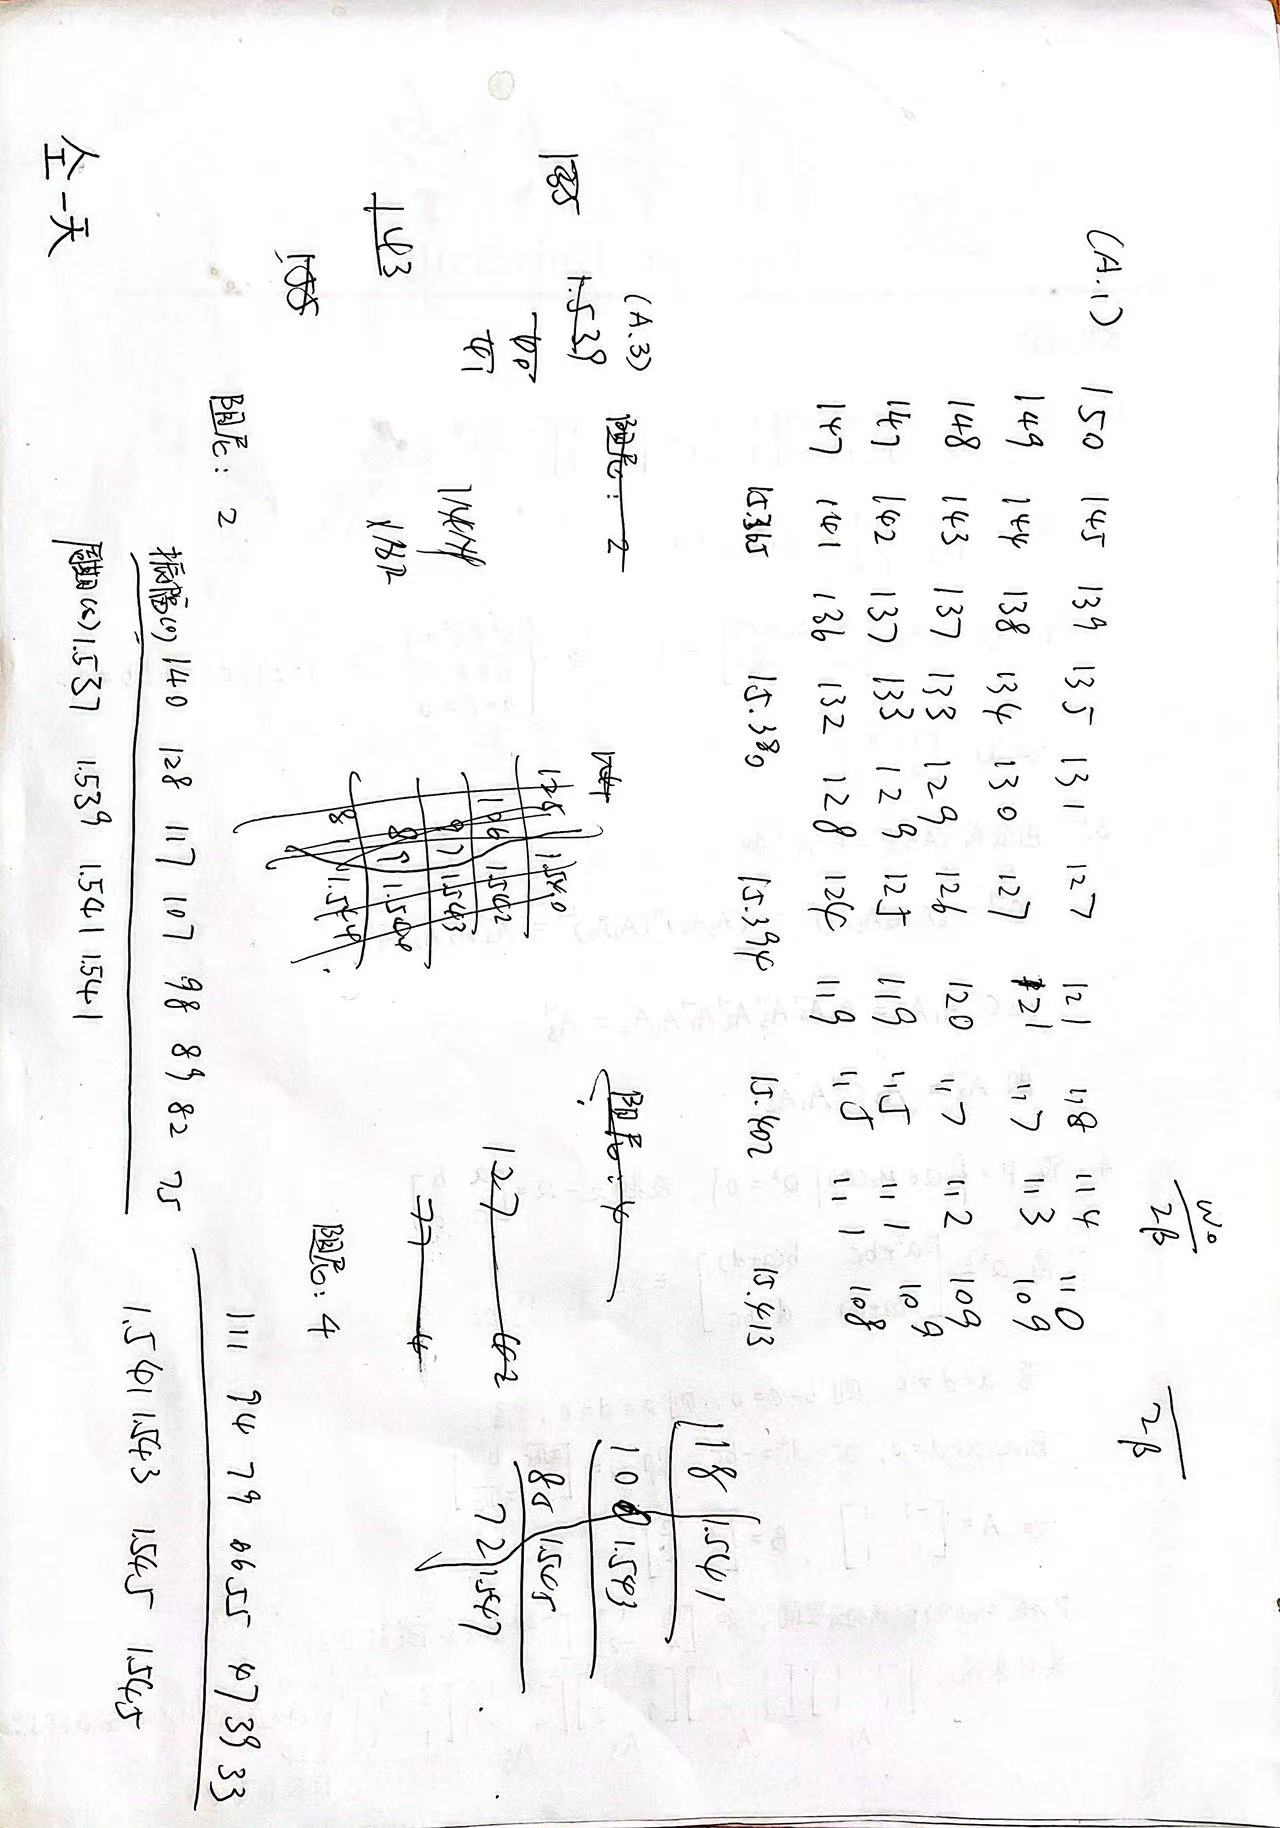
\includegraphics[width=.95\linewidth]{原始数据1.jpg}
\end{figure}

\begin{figure}[h]
	\centering
	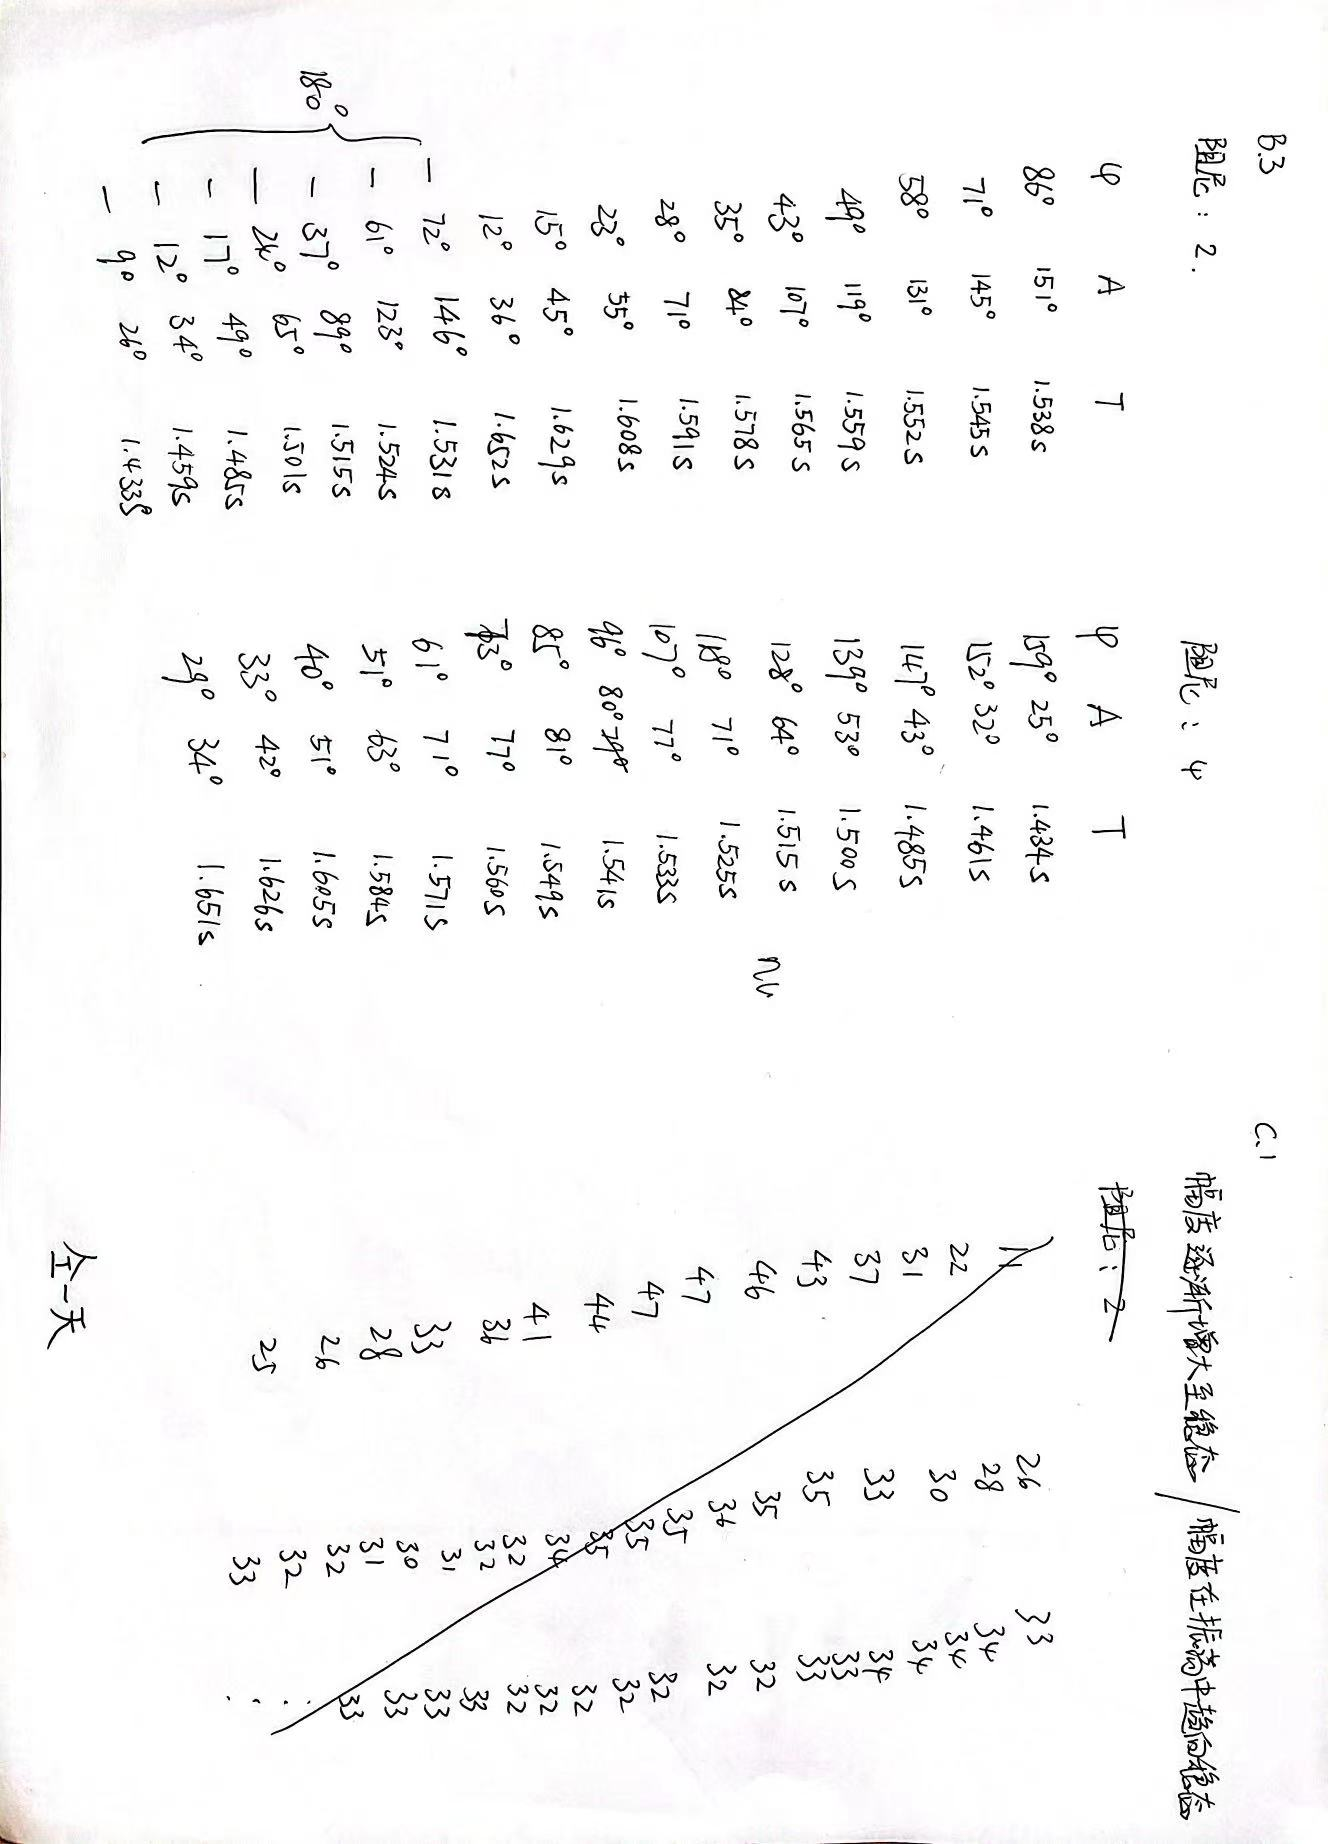
\includegraphics[width=.95\linewidth]{原始数据2.jpg}
\end{figure}

\begin{figure}[h]
	\centering
	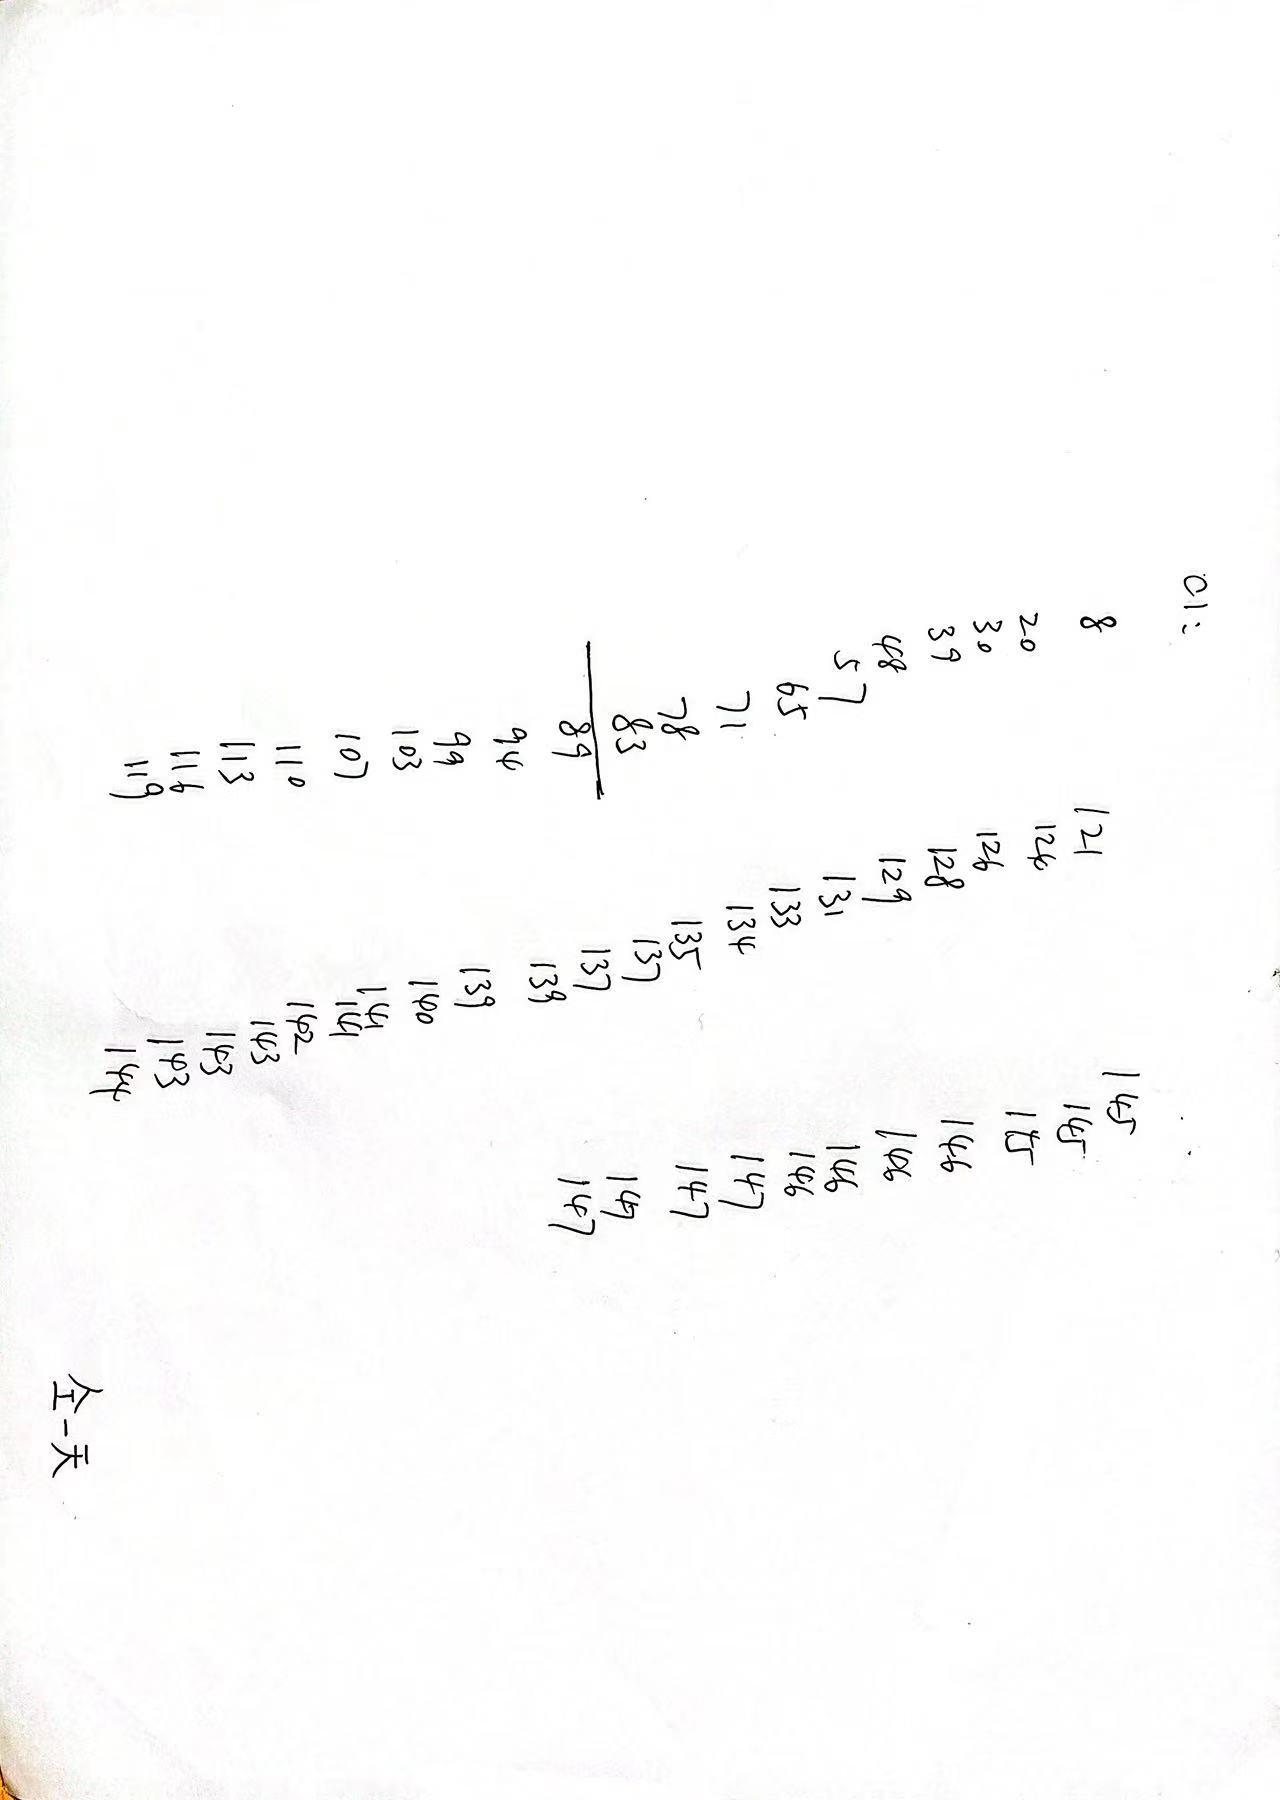
\includegraphics[width=.95\linewidth]{原始数据3.jpg}
\end{figure}
\vfill\noindent\itshape\footnotesize
\end{document}
